\RequirePackage{plautopatch}
\documentclass[a4paper,12pt,dvipdfmx]{jlreq}
%英語フォント
\usepackage{tgtermes,tgheros,tgcursor}
%日本語を多書体にする
\usepackage{jlreq-deluxe}
%数式用
\usepackage{amsmath}
\usepackage[varg]{newtxmath}
\newcommand{\symbb}{\vvmathbb}
%日本語太字を戻すためのおまじない
\renewcommand{\bfdefault}{bx}
%図のとりこみ
\usepackage{graphicx}
\usepackage{physics}
%文献
\usepackage{hep-bibliography}
\bibliography{ref.bib}

\newcommand{\Zb}{\mathbb{Z}}
\newcommand{\Kt}{\widetilde{K}}
\newcommand{\ZIs}{Z_{\mathrm{Ising}}}
\newcommand{\ZGIs}{Z_{\mathrm{Ising}/\mathbb{Z}_2}}
\newcommand{\deltamod}{\delta^{\mathrm{mod}\ 2}}

\begin{document}

\begin{center}
  \textbf{\sffamily \LARGE 2次元Ising模型のKramers-Wannier双対性}
\end{center}

\begin{flushright}
  \textbf{\sffamily \Large 山口 哲}  
\end{flushright}

\section{導入}
このノートでは2次元Ising模型のKramers-Wannier (KW) 双対性\cite{Kramers:1941kn,Kramers:1941zz}の導出をまとめている。

もちろんKW双対性の導出は少し詳しい目の統計力学の教科書に出ている。それこのノートであらためてまとめておこうと思ったのは2つの理由がある。

1つは熱力学極限だけでなく、精密な双対性について述べたかったからである。
もちろんIsing模型の相転移点の決定などに使う場合には熱力学極限だけで十分である。
しかし、最近のトポロジカルな議論に使う場合には、離散対称性のゲージ化に関する精密な議論が必要である。
ここではそれも含めて導出する。

もう一つは高次元への一般化を紹介したかったからである\cite{Wegner:1971app}。
こちらも最近のトポロジカルな議論での良いモデルになる。

Ising模型は次のようなものである。2次元の正方格子を考える。ここでは有限の格子でトーラス状に周期境界条件が課されているとする。サイトのラベルを$i,j$とする。各サイトに「スピン」の自由度$a_{i}=0,1$を置く。各リンクを両端のサイトのラベル$i,j$を用いて$\expval{ij}$のように表す。定数のパラメーターを$K>0$としてイジング模型の分配関数は
\begin{align}
  \ZIs(K)=\sum_{\{a\}} \exp\left(
    K\sum_{\expval{ij}:\text{すべてのリンク} }(-1)^{a_i+a_j}
  \right).
\end{align}
ここで$\sum_{\{a\}}$はすべてのスピンの配位についての和である。

一方で、Ising模型の$\Zb_2$対称性をゲージ化した模型の分配関数は、
\begin{align}
  \ZGIs(K)=\frac12 \sum_{\text{boundary conditions}}
  \sum_{\{a\}}\exp\left(
    K\sum_{\expval{ij}:\text{すべてのリンク} }(-1)^{a_i+a_j}
  \right)
  \label{Ising/Z2}
\end{align}
となる。ここで$\sum_{\text{boundary conditions}}$はトーラスの2つの周期の方向の境界条件を周期境界条件か反周期境界条件のどちらかを選ぶ4通りの境界条件についての和である。弦理論をご存知の方は、「オービフォールド」の操作をしたものである。

Kramers-Wannier双対性の厳密な表式は
\begin{align}
  \frac{1}{(\sinh 2K)^{2V}}\ZGIs(K)=
  \frac{1}{(\sinh 2\Kt)^{2V}}\ZIs(\Kt)
  \label{KWduality}
\end{align}
である。因子$\frac{1}{(\sinh 2K)^{2V}}$は局所的な項として作用に入れることができる。したがって、この式は二つの系の等価性を表している。このノートの目的は、この式の証明を与えることと、その高次元の対応物について説明することである。

\section{Kramers-Wannier双対性の導出}
証明に関して次のような系を考える。まず、各リンク$\ell$に自由度$b_{\ell}=0,1$を置く。また、各プラケット$p$に自由度$c_{p}$を置く。その分配関数を
\begin{align}
  Z(K)=\sum_{\{b\}}\frac{1}{2^{V}} \exp\left[
    K\sum_{\ell:\text{links}}(-1)^{b_{\ell}}+i\pi\sum_{\substack{p=\expval{\ell_1 \ell_2 \ell_3 \ell_4}:\\ \text{plaquettes}}} c_{p}(b_{\ell_1}+b_{\ell_2}+b_{\ell_3}+b_{\ell_4})
  \right]
  \label{model1}
\end{align}
とする。$p=\expval{\ell_1 \ell_2 \ell_3 \ell_4}$はプラケット$p$を構成する4辺が$\ell_1, \ell_2, \ell_3, \ell_4$ということである。

方針としては、式\eqref{model1}を二つのやり方で変形したのが、大雑把に言って\eqref{KWduality}の左辺と右辺となる。

\subsection{第1の変形}
第1の変形では、まず$c$についての和を評価する。用いる式は整数$b$に対して 
\begin{align}
  \frac12\sum_{c=0,1}\exp(i\pi c b )
  =\deltamod_{b,0}
  :=
  \begin{cases}
    1& (b=0 \mod 2)\\
    0& (b=1 \mod 2)
  \end{cases}
\end{align}
という恒等式である。この式を用いると
\begin{align}
  Z(K)=\sum_{\{b\}}\frac{1}{2^{V}} \exp\left[
    K\sum_{\ell:\text{links}}(-1)^{b_{\ell}}
    \right]
    \prod_{\substack{p=\expval{\ell_1 \ell_2 \ell_3 \ell_4}:\\ \text{plaquettes}}} \deltamod_{b_{\ell_1}+b_{\ell_2}+b_{\ell_3}+b_{\ell_4}}
    \label{model1-1-1}
\end{align}
を得る。

式\eqref{model1-1-1}から、寄与が$0$でない$b_{\ell}$の配位は各サイトに置いたスピン$a_{i}$と「だいたい」1対1対応していることが次のように分かる。
\begin{itemize}
  \item 与えられた$a_{i}$の配位に対して$b_{\expval{ij}}=a_i-a_j \mod 2$とすれば、プラケットが$0$の$b$の配位が得られる。
  \item 逆にプラケットがすべて$0$である$b_{\ell}$の配位から次のようにして$a_{i}$の配位を得る。原点のサイト$0$を一つ固定する。図\ref{fig:path}のようにサイト$0$からサイト$i$までのリンク$\ell_1,\ell_2,\dots,\ell_N$を辿っていく経路をとり、
  \begin{align}
    a_{i}=a_{0}+b_{\ell_1}+b_{\ell_2}+\dots+b_{\ell_N} \mod 2
  \end{align}
  で与える。$b$のプラケットがすべて$0$なので、経路のプラケット1つ分の変形、そしてそれを繰り返して得られる変形で不変である。
\end{itemize}
\begin{figure}[htbp]
  \centering
  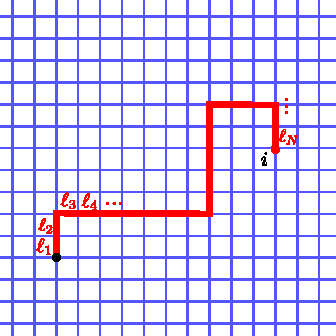
\includegraphics{path.pdf}
  \caption{{}}
  \label{fig:path}
\end{figure}

「だいたい」と言ったのは、次の2点で1対1対応では無いからである。
\begin{itemize}
  \item $b$の配位を決めたとき、$a_0$の値は任意である。つまり、$b$の配位を決めたとき、対応する$a$の配位は2種類ある。
  \item $b$から$a$を作るとき、経路によらないわけではない。プラケット1つ分の変形を繰り返すことでは繋がらない経路がある。この経路への依存性は、非自明なサイクルでの$b$の和の偶奇で特徴づけられる。つまり、$b$の配位と対応する$a$の配位は非自明なサイクルに関して周期境界条件あるいは反周期境界条件を持つものすべてを考えなければならない。
\end{itemize}
これらを正しく考慮すると
\begin{align}
  Z(K)=\ZGIs(K)
\end{align}
を得る。式\eqref{Ising/Z2}の$\ZGIs(K)$で全体にかかっている$1/2$が前者からくるもの、境界条件に関する和が後者から来るものである。

\subsection{第2の変形}



\subsection{双対性のまとめ}

\section{双対性からの帰結}

\section{高次元への一般化}

\printbibliography
\end{document}